\chapter{Designing the Architecture}
Following The Von Neumann the architecture shall be structured in a number of modules, the arithmetic logic unit, the control unit, memory, input and output. The modules interact with each over the three buses, sharing data, address and control signals. All actions are orchestrated by the control unit, signalling the other modules when to read or write data, when to perform calculations, and when to output data, based on the micro instructions stored in the control unit.

When taking into account that (random access) memory retrieval takes significantly longer than any other operation the von Neumann bottleneck can be alleviated to a certain extent by introducing a secondary, faster, form of memory. Deviating from the von Neumann Architecture the memory module shall be split up into to two modules, a random access memory, storing data and instructions referenced by addresses and the registers, storing only a single bus width (a data word). As well as a number of registers, storing operand data for the arithmetic logic unit. The registers function without an address and are directly operated by the control unit.

The modules, in which this architecture is split up to, thus are the ALU, the CU, the memory, the register
and the input and output.
\begin{figure}[H]
  \begin{center}
    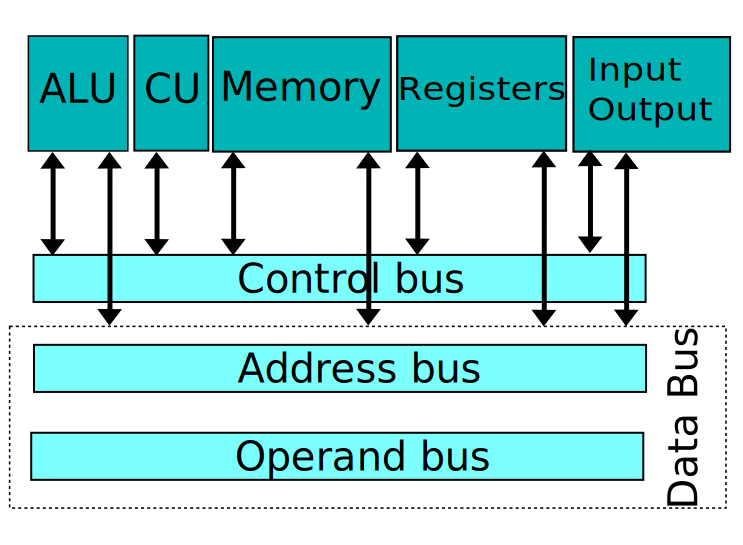
\includegraphics[width=0.5\textwidth]{figures/VNA-Adapted}
  \end{center}
  \caption{The Von Neumann Architecture. Adapted from \cite{fig-vna}}\label{fig:vna-adapted}
\end{figure}


Given the previously defined goal \ref{sec:goals} three distinct groups of requirements to the computer architecture can be differentiated. Requirements resulting from the need for Turing equivalence are from here on out referred to as "Turing requirements".

Architectural requirements are a set of non-functional requirements given by the intended computer architecture. They are by design only verifiable and not testable.

Finally, feature requirements are requirements that are arbitrarily defined by me to expand the feature set. These requirements shall be justified, when put in place and tested.

Requirements are inlined and numbered to provide a point of reference when implementing and testing the requirements in the simulation. 

\newtheorem{turing-requirement}{Turing Req.}[section]
\newtheorem{arch-requirement}{Arch. Req.}[section]
\newtheorem{feat-requirement}{Feat. Req.}[section]

The keywords "must", "must not", "required", "shall", "shall not", "should", "should not", "recommended",  "may", and "optional" in the requirements are to be interpreted as described in RFC 2119 \cite{rfc2119}.


\section{Arithmetic Logic Unit}
The Arithmetic Logic Unit is the module performing all arithmetic and logical operations on operands. It
is the centerpiece of the computer, as it is the only module that modifies, or synthesizes, new data.

The most commonly used and implemented arithmetic operation is addition and thus shall be the first operation to be implemented.
\begin{turing-requirement}
  Ability to add two data words.
\end{turing-requirement}

To source ideas for additional features and operations ChatGPT was harnessed to generate a few. From a number of suggestions, I decided to implement subtraction, shift, rotation and bit shift operations shall be implemented. It additionally suggested features such as floating point math, vector math, multiplication and division. Multiplication and division however shall not be implemented, as these operations are not performable in a single iteration \cite{chatgptalu}.
Binary multiplication is normally achieved by repeated addition of the multiplicand to itself, whilst counting the addition operations, stopping when the multiplier is reached. The simplest way of performing a division, specifically integer division, is by repeated subtraction of the divisor from the dividend until a number smaller than the divisor is reached. As the architecture implements repeatable operations based on conditions, multiplication and division can be performed in macro code. This would be redundant.

Likewise, rotation and shift operations shall only be implemented for a single bit, as any other shift or rotation can only be achieved by performing the shift multiple times or by having multiple shift and rotate circuits in series.
\begin{feat-requirement}
  Ability to subtract two data words.
\end{feat-requirement}

\begin{feat-requirement}
  Ability to shift a data word bitwise.
\end{feat-requirement}

\begin{feat-requirement}
  Ability to rotate a data word bitwise.
\end{feat-requirement}

\begin{feat-requirement}
  Ability to AND, OR and XOR two data words.
\end{feat-requirement}

\begin{feat-requirement}
  Ability to NOT a data word.
\end{feat-requirement}

Furthermore, the computer is required to be able to execute conditionally, thus requiring a data point indicating if a condition is true or not. This indication is called a flag. The two most common flags are the zero flag and the carry flag, as they are easily generated mathematically. 

The carry flag, which indicates whether or not an addition in the ALU has overflown, so resulted in a number which is larger than the 8-bit data word size. Apart from being useful in conditional jumps, the carry flag can also be used to detect if a calculation has overflown, and thus if the result is incorrect.

\begin{turing-requirement}
  Generation of a carry flag. 
\end{turing-requirement}

The zero flag indicates if the result of an operation is zero. This is not only useful for looping a fixed number of times, but also for comparing two data words. As the ALU is designed to subtract two data words, a zero flag allows for easy determination if two data words are equal, by subtracting them from each other. 

\begin{feat-requirement}
  Generation of a zero flag.
\end{feat-requirement}

Given the fact that the architecture has an 8-bit data bus, and the ALU performing 8-bit operations, the ALU will always need to buffer the two operands. Instead of having the ALU buffer the operands, with two additional registers, the ALU shall access two registers directly, that are otherwise, independent of the ALU.
\begin{arch-requirement}
  Ability to take in data from 2 registers.
\end{arch-requirement}

As the calculation results need to return to registers and memory, the ALU must have the ability to output data to the bus.
\begin{arch-requirement}
  Ability to output operation results to the bus. 
\end{arch-requirement}

Finally, the ALU shall not exert undefined behaviour in case of undefined control signals, and shall not output unless control signals indicate to do so. 

\begin{feat-requirement} \label{req:alu-undef-behavior}
  Must not exert undefined behaviours in case of undefined control signals. 
\end{feat-requirement}

\begin{feat-requirement} \label{req:alu-no-output}
  Must not output unless control signals indicated to do so. 
\end{feat-requirement}

\section{Memory}

\begin{turing-requirement}
Must allow writing to and reading from a memory location
\end{turing-requirement}

As instructions need data to operate on, the data, operands, and instructions should ideally be stored in a way that allows accessing one together with the other. The simplest approach would be to transfer the instruction together with the operand on to the bus, as in the SAP-2 architecture \cite{malvino1983a}.

As an 8-bit bus width is required, equally splitting the bus into 4 bits for the instruction and 4 bits for the operand would be the most straightforward approach.

This however results in only 16 possible instructions and the highest possible operand value of 15. Although this would not impact turing completeness or any other requirement, it does not allow for an easily usable instruction set. In fact, manual programming of any "complex" task would be very difficult. One could achieve higher instruction count by reserving one instruction for all non-operand instructions and then using the last 4 bits to identify the individual instruction. This would allow for 31 instructions, 15 of which with operands up to 15.

Increasing the size of the instruction or operand is no option either as the other component would need to shrink, resulting in the architecture either having less instructions or smaller operands.

A solution to this problem is the introduction of a second data word that is stored in memory alongside, essentially increasing the address bus width by one but instead but running this wire as part of the control bus. The indication of which data word is thus tied to the instruction's microprogramming and is not intended to be chosen at runtime. Additionally this way of increasing the address bus does not require running a wire to every component, keeping the physical layout simple. Finally the size of the stored programm is also smaller, as the indication of the used data word is only stored once in the microcode contrary to repetitvely storing it in the program code.  

As the active data word must be configured per microinstruction, before computer execution specifying each data word, each data word is assigned a purpose. The first one storing the instruction and the second storing the operand.    

\begin{feat-requirement}
Must store, for each memory address, store two data words. A control signal shall indicate which data word to access. The first data word shall be intended for instructions and the second for operands.
\end{feat-requirement}

While an 8 bit operand is considered sufficient for this architecture a program with only 255 instruction steps is not. Furthermore, to make the architecture Turing complete the architecture needs to be able to address infinite memory. To realize this, the primary addressing mode shall be relative. Additionally, the address width of the memory shall be extendable beyond the width of the 8-bit bus.

\begin{feat-requirement}
Must retrieve data with a relative memory address. 
\end{feat-requirement}

To allow for relative addressing, the program counter (PC) must be stored in full length. Additionally, to allow useful programming a second general purpose memory address register (MAR) shall be implemented. % TODO: Explain better

\begin{feat-requirement}
Must store the program counter and memory address register.
\end{feat-requirement}

For certain features, such as a call stack, it is nonetheless useful to allow for abosulte addressing. Additionally, first $8$-bit of the PC and MAR shall be overwriteable for absolute access but with an offset. 

\begin{feat-requirement}
Must retrieve data with an absolute memory address. 
\end{feat-requirement}


When the program is executed the first micro instruction will always be to increment the PC to get the next instruction. As that one cannot come from the bus, as no instruction or memory is present, the PC must be able to be incremented without the bus.
\begin{feat-requirement}
    Must be able to increment the program counter by one with a specific control signal.
\end{feat-requirement}

\iffalse
With relative jumps of only 255 but bigger word counts. 
Assembler could impl like jump over 

PSEUDO
NORMAL PROGRAM
JMP2
JPD 255 
NORMAL PROGRAM RESUMES HERE
.
.
.
SOME OTHER PROGRAM THAT NEEDS TO JUMP MORE THAN ONE

\fi

\section{Registers}
As established in the architecture, the computer shall have a set of registers to store data words. The registers shall be able to store data words and output them to the bus.

\begin{feat-requirement}
  Ability to load a data word for storage.
\end{feat-requirement}

\begin{feat-requirement}
  Ability to output a data word.
\end{feat-requirement}

The registers must also directly interface with the ALU, by providing direct access without any control signals. 

\begin{arch-requirement} \label{req:register-direct-access}
  Must be able to be read by the ALU without any control signals.
\end{arch-requirement}


\section{Control Unit}
Following the VNA the module orchestrating the interaction and operation of all modules is called the Control Unit. It is responsible for the generation of the control word, based on the macro program, the current state of the computer and current timing information. For every given combination of input the control word must produce a specific output forming a truth table. In historic computer architectures this truth table was represented by carefully creating a net of logic gates, which would produce the correct output for every input, to satisfy the truth table. With the increasing complexity and the fact that once physically produced this control logic could not be changed, the concept of the microcode was invented \cite{cite.needed}. A storage, given enough address and data bus width, can represent any truth table, just like a combination of logic gates, with the key advantage of being reprogrammable. Thus, nowadays, control units are often not more than a piece of storage and a timing unit. If a silicon design is not intended to be micro-(re)-programmable, the storage/truth table can be minimized with certain algorithms and then hardwired into the silicon. As representing the truth table in a storage is the most flexible way, the control unit shall be implemented as a microcode storage.

\begin{arch-requirement}
  The microcode shall be implemented as storage.
\end{arch-requirement}

\begin{arch-requirement} \label{req:cw-from-instr}
  Must produce the control word (micro instruction) from instruction and state.
\end{arch-requirement}

To achieve Turing completeness, the control unit must be able to handle conditional operations based on the flags, as the flags represent all the architectures intended conditions.

\begin{turing-requirement}
  Must produce the control word from flags.
\end{turing-requirement}



\begin{arch-requirement}
  Must produce the clock signal. 
\end{arch-requirement}

Each clock cycle shall be counted to produce the \textit{timing state} count. A timing state is the time frame in which one micro instruction is executed. The number of timing states is determined by the number of micro instructions needed to execute an instruction. The number of required timing states, so the amount of microinstructions comprising one macro instruction, can only be determined once the exact instruction set is defined. Thus, the space needed in the control word for the timing state can only be estimated for now. Given that the instruction set is not yet defined, checking the seemingly most complex instruction, a jump instruction, is a good starting point. 

The required states for a basic jump instruction already are: 
\begin{enumerate}
  \item Increment PC
  \item Fetch instruction (for certain jumps, only if the flags are set correctly)
  \item Fetch second data word (instruction argument) and increment program counter by it.
  \item Fetch instruction from new program counter
  \item Execute the new instruction
\end{enumerate}
    
As the execution of the new jumped to instruction will probably take more than one step, the total count of timing states is thus is 6-8. Given that the timing state is represented in binary, the smallest number of bits needed to represent 8 states is 3. However, to ensure that the control unit coulf be used for more complex instructions, the number of timing states shall be set to 16 (4 bits).

\begin{arch-requirement}
  Must count clock cycles to produce 16 timing states and reset to zero once 16 was reached or the control word indicated to do so.
\end{arch-requirement}

To compensate for any redundant timing states a microcode signal to break out of the current instruction and skip to the next one is needed. The 

\begin{feat-requirement}
  Must, given a specific output of the microcode break out of the current instruction (reset state signal).
\end{feat-requirement}


Given that for the computer to function every instruction must be first pointed to by the program counter and then loaded into the control unit, the relevant control words must be setup in the microcode. Instead of hard coding this into the control unit this shall be part of the standard microcode generation process.
\begin{feat-requirement}
  The control word generated by the first state, regardless of flag and macro instruction, must always increment the program counter by one. 
\end{feat-requirement}

\begin{feat-requirement}
  The control word generated by the second state, regardless of flag and macro instruction, must always fetch the current instruction and store it in the macro instruction register.
\end{feat-requirement}


\begin{feat-requirement}
  Must halt given micro/macrocode instruction to do so. 
\end{feat-requirement}

\section{Input and Output}
This architecture shall not specifically implement any input and output capabilities, as they are not required as per \ref{sec:goals}. Any input or output can be handled by test benches, either by storing directly into memory cells or into registers.